%{{第七十二回}}{第七十二回}}
\chapter{王熙凤恃强羞说病\\来旺妇倚势霸成亲}

{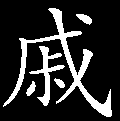
\includegraphics[width=3mm]{../Images/00005}\kaishu 此回似着意似不着意,似接续似不接续,在画师为浓淡相间,在墨客为骨肉停匀,在乐工为笙歌间作,在文坛为养局为别调。前后文气,至此一歇。}

且说鸳鸯出了角门,脸上犹红,心内突突的,真是意外之事。因想这事非常,若说出来,奸盗相连,关系人命,还保不住带累了旁人。横竖与自己无干,且藏在心内,不说与一人知道。回房复了贾母的命,大家安息。从此凡晚间便不大往园中来。\elegantpar{因思园中尚有这样奇事}{所谓脏唐臭汉},何况别处,因此连别处也不大轻走动了。

原来那司棋因从小儿和他姑表兄弟在一处顽笑起住时,小儿戏言,便都订下将来不娶不嫁。近年大了,彼此又出落的品貌风流。常时司棋回家时,二人眉来眼去,旧情不忘,只不能入手。又彼此生怕父母不从,二人便设法彼此里外买嘱园内老婆子们留门看道,今日趁乱方初次\elegantpar{入港}{秦钟}。虽未成双,却也海誓山盟,私传表记,已有无限风情了。忽被鸳鸯惊散,那小厮早穿花度柳,从角门出去了。司棋一夜不曾睡着,又后悔不来。直至次日见了鸳鸯,自是脸上一红一白,百般过不去。心内怀着鬼胎,茶饭无心,起坐恍惚。挨了两日,竟不听见有动静,方略放下了心。这日晚间,忽有个婆子来悄告诉他道:``你兄弟竟逃走了,三四天没归家。如今打发人四处找他呢。''司棋听了,气个倒仰,因思道:``纵是闹了出来,也该死在一处。他自为是男人,先就走了,可见是个没情意的。''因此又添了一层气。次日便觉心内不快,百般支持不住,一头睡倒,恹恹的成了大病。

鸳鸯闻知那边无故走了一个小厮,园内司棋又病重,要往外挪,心下料定是二人惧罪之故,``生怕我说出来,方吓到这样。''因此自己反过意不去,指着来望候司棋,支出人去,反自己立身发誓,与司棋说:``我告诉一个人,立刻现死现报!你只管放心养病,别白糟踏了小命儿。''司棋一把拉住,哭道:``我的姐姐,咱们从小儿耳鬓厮磨,你不曾拿我当外人待,我也不敢待慢了你。如今我虽一着走错,你若果然不告诉一个人,你就是我的亲娘一样。从此后我活一日是你给我一日,我的病好之后,把你立个长生牌位,我天天焚香礼拜,保佑你一生福寿双全。我若死了时,变驴变狗报答你。再俗语说:`千里搭长棚,没有不散的筵席。'再过三二年,咱们都是要离这里的。俗语又说:`浮萍尚有相逢日,人岂全无见面时。'倘或日后咱们遇见了,那时我又怎么报你的德行。''一面说,一面哭。这一席话反把鸳鸯说的心酸,也哭起来了。因点头道:``正是这话。我又不是管事的人,何苦我坏你的声名,我白去献勤。况且这事我自己也不便开口向人说。你只放心。从此养好了,可要安分守己,再不许胡行乱作了。''司棋在枕上点首不绝。

鸳鸯又安慰了他一番,方出来。因知贾琏不在家中,又因这两日凤姐儿声色怠惰了些,不似往日一样,因顺路也来望候。因进入凤姐院门,二门上的人见是他来,便立身待他进去。鸳鸯刚至堂屋中,只见平儿从里间出来,见了他来,忙上来悄声笑道:``才吃了一口饭歇了午睡,你且这屋里略坐坐。''鸳鸯听了,只得同平儿到东边房里来。小丫头倒了茶来。鸳鸯因悄问:``你奶奶这两日是怎么了?我看他懒懒的。''平儿见问,因房内无人,便叹道:``他这懒懒的也不止今日了,这有一月之前便是这样。又兼这几日忙乱了几天,又受了些闲气,从新又勾起来。这两日比先又添了些病,所以支持不住,便露出马脚来了。''鸳鸯忙道:``既这样,怎么不早请大夫来治?''平儿叹道:``我的姐姐,你还不知道他的脾气的。别说请大夫来吃药。我看不过,白问了一声身上觉怎么样,他就动了气,反说我咒他病了。饶这样,天天还是察三访四,自己再不肯看破些且养身子。''鸳鸯道:``虽然如此,到底该请大夫来瞧瞧是什么病,也都好放心。''平儿道:``我的姐姐,说起病来,据我看也不是什么小症候。''鸳鸯忙道:``是什么病呢?''平儿见问,又往前凑了一凑,向耳边说道:``只从上月行了经之后,这一个月竟沥沥淅淅的没有止住。这可是大病不是?''鸳鸯听了,忙答道:``嗳哟!依你这话,这可不成了血山崩了。''平儿忙啐了一口,又悄笑道:``你女孩儿家,这是怎么说的,倒会咒人呢。''鸳鸯见说,不禁红了脸,又悄笑道:``究竟我也不知什么是崩不崩的,你倒忘了不成,先我姐姐不是害这病死了。我也不知是什么病,因无心听见妈和亲家妈说,我还纳闷,后来也是听见妈细说原故,才明白了一二分。''平儿笑道:``你该知道的,我竟也忘了。''

二人正说着,只见小丫头进来向平儿道:``方才朱大娘又来了。我们回了他奶奶才歇午觉,他往太太上头去了。''平儿听了点头。鸳鸯问:``那一个朱大娘?''平儿道:``就是官媒婆那朱嫂子。因有什么孙大人家来和咱们求亲,所以他这两日天天弄个帖子来赖死赖活。''一语未了,小丫头跑来说:``二爷进来了。''说话之间,贾琏已走至堂屋门,口内唤平儿。平儿答应着才迎出来,贾琏已找至这间房内来。至门前,忽见鸳鸯坐在炕上,便煞住脚,笑道:``鸳鸯姐姐,今儿贵脚踏贱地。''鸳鸯只坐着,笑道:``来请爷奶奶的安,偏又不在家的不在家,睡觉的睡觉。''贾琏笑道:``姐姐一年到头辛苦伏侍老太太,我还没看你去,那里还敢劳动来看我们。正是巧的很,我才要找姐姐去。因为穿着这袍子热,先来换了夹袍子再过去找姐姐,不想天可怜,省我走这一趟,姐姐先在这里等我了。''一面说,一面在椅上坐下。

鸳鸯因问:``又有什么说的?''贾琏未语先笑道:``因有一件事,我竟忘了,只怕姐姐还记得。上年老太太生日,曾有一个外路和尚来孝敬一个蜡油冻的佛手,因老太太爱,就即刻拿过来摆着了。因前日老太太生日,我看古董账上还有这一笔,却不知此时这件东西着落何方。古董房里的人也回过我两次,等我问准了好注上一笔。所以我问姐姐,如今还是老太太摆着呢,还是交到谁手里去了呢?''鸳鸯听说,便道:``老太太摆了几日厌烦了,就给了你们奶奶。你这会子又问我来。我连日子还记得,还是我打发了老王家的送来的。你忘了,或是问你们奶奶和平儿。''平儿正拿衣服,听见如此说,忙出来回说:``交过来了,现在楼上放着呢。奶奶已经打发过人出去说过给了这屋里,他们发昏,没记上,又来叨登这些没要紧的事。''贾琏听说,笑道:``既然给了你奶奶,我怎么不知道,你们就昧下了。''平儿道:``奶奶告诉二爷,二爷还要送人,奶奶不肯,好容易留下的。这会子自己忘了,倒说我们昧下。那是什么好东西,什么没有的物儿。比那强十倍的东西也没昧下一遭,这会子爱上那不值钱的!''贾琏垂头含笑想了一想,拍手道:``我如今竟糊涂了!丢三忘四,惹人抱怨,竟大不像先了。''鸳鸯笑道:``也怨不得。事情又多,口舌又杂,你再喝上两杯酒,那里清楚的许多。''一面说,一面就起身要去。

贾琏忙也立身说道:``好姐姐,再坐一坐,兄弟还有事相求。''说着便骂小丫头:``怎么不潗好茶来!快拿干净盖碗,把昨儿进上的新茶潗一碗来。''说着向鸳鸯道:``这两日因老太太的千秋,所有的几千两银子都使了。几处房租地税通在九月才得,这会子竟接不上。明儿又要送南安府里的礼,又要预备娘娘的重阳节礼,还有几家红白大礼,至少还得三二千两银子用,一时难去支借。俗语说,`求人不如求己'。\elegantpar{说不得,姐姐担个不是,暂且把老太太查不着的金银家伙偷着运出一箱子来,暂押千数两银子支腾过去。不上半年的光景,银子来了,我就赎了交还,断不能叫姐姐落不是。}{起风波}''鸳鸯听了,笑道:``你倒会变法儿,亏你怎么想来。''贾琏笑道:``不是我扯谎,若论除了姐姐,也还有人手里管的起千数两银子的,只是他们为人都不如你明白有胆量。我若和他们一说,反吓住了他们。所以我`宁撞金钟一下,不打破鼓三千'。''一语未了,忽有贾母那边的小丫头子忙忙走来找鸳鸯,说:``老太太找姐姐半日,我们那里没找到,却在这里。''鸳鸯听说,忙的且去见贾母。

贾琏见他去了,只得回来瞧凤姐。谁知凤姐已醒了,听他和鸳鸯借当,自己不便答话,只躺在榻上。听见鸳鸯去了,贾琏进来,凤姐因问道:``他可应准了?''贾琏笑道:``虽然未应准,却有几分成手,须得你晚上再和他一说,就十分成了。''凤姐笑道:``我不管这事。倘或说准了,这会子说得好听,到有了钱的时节,你就丢在脖子后头,谁去和你打饥荒去。倘或老太太知道了,倒把我这几年的脸面都丢了。''贾琏笑道:``好人,你若说定了,我谢你如何?''凤姐笑道:``你说,谢我什么?''贾琏笑道:``你说要什么就要什么。''平儿一旁笑道:``奶奶倒不要谢的。昨儿正说要作一件什么事,恰少一二百银子使,不如借了来,奶奶拿一二百银子,岂不两全其美。''凤姐笑道:``幸亏提起我来,就是这样也罢。''贾琏笑道:``你们太也狠了。你们这会子别说一千两的当头,就是现银子要三五千,只怕也难不倒。我不和你们借就罢了。这会子烦你说一句话,还要个利钱,真真了不得。''凤姐听了,翻身起来说:``我有三千五万,不是赚的你的。如今里里外外上上下下背着我嚼说我的不少,就差你来说了,可知没家亲引不出外鬼来\href{../Text/part0076_split_000.html\#lnkback_1_a}{\textsuperscript{①}}。我们王家可那里来的钱,都是你们贾家赚的。别叫我恶心了。你们看着你们家,什么石崇、邓通!把我王家的地缝子扫一扫,就够你们过一辈子呢。说出来的话也不怕臊!\elegantpar{现有对证:把太太和我的嫁妆细看看,比一比你们的,那一样是配不上你们的。}{贾家王家联姻}''贾琏笑道:``说句顽话就急了。这有什么这样的,要使一二百两银子值什么,多的没有,这还有,先拿进来,你使了再说,如何?''凤姐道:``我又不等着衔口垫背,忙了什么。''贾琏道:``何苦来,不犯着这样肝火盛。''凤姐听了,又自笑起来,``不是我着急,你说的话戳人的心。我因为我想着后日是尤二姐的周年,我们好了一场,虽不能别的,到底给他上个坟烧张纸,也是姊妹一场。他虽没留下个男女,也要\href{../Text/part0076_split_000.html\#lnkback_2_a}{\textsuperscript{②}}`前人撒土迷了后人的眼'才是。''一语倒把贾琏说没了话,低头打算了半晌,方道:``难为你想的周全,我竟忘了。既是后日才用,若明日得了这个,你随便使多少就是了。''

一语未了,只见旺儿媳妇走进来。凤姐便问:``可成了没有?''旺儿媳妇道:``竟不中用。我说须得奶奶作主就成了。''贾琏便问:``又是什么事?''凤姐儿见问,便说道:``不是什么大事。旺儿有个小子,今年十七岁了,还没得女人,因要求太太房里的彩霞,不知太太心里怎么样,就没有计较得。前日太太见彩霞大了,二则又多病多灾的,因此开恩打发他出去了,给他老子娘随便自己拣女婿去罢。因此旺儿媳妇来求我。我想他两家也就算门当户对的,一说去自然成的,谁知他这会子来了,说不中用。''贾琏道:``这是什么大事,比彩霞好的多着呢。''旺儿家的陪笑道:``爷虽如此说,连他家还看不起我们,别人越发看不起我们了。好容易相看准一个媳妇,我只说求爷奶奶的恩典,替作成了。奶奶又说他必肯的,我就烦了人走过去试一试,谁知白讨了没趣。若论那孩子倒好,据我素日私意儿试他,他心里没有甚说的,只是他老子娘两个老东西太心高了些。''一语戳动了凤姐和贾琏,凤姐因见贾琏在此,且不作一声,只看贾琏的光景。贾琏心中有事,那里把这点子事放在心里。待要不管,只是看着他是凤姐儿的陪房,且又素日出过力的,脸上实在过不去,因说道:``什么大事,只管咕咕唧唧的。你放心且去,我明儿作媒打发两个有体面的人,一面说,一面带着定礼去,就说我的主意。他十分不依,叫他来见我。''旺儿家的看着凤姐,凤姐便扭嘴儿。旺儿家的会意,忙爬下就给贾琏磕头谢恩。

贾琏忙道:``你只给你姑娘磕头。我虽如此说了这样行,到底也得你姑娘打发个人叫他女人上来,和他好说更好些。虽然他们必依,然这事也不可霸道了。''凤姐忙道:``连你还这样开恩操心呢,我倒反袖手旁观不成。旺儿家你听见,说了这事,你也忙忙的给我完了事来。说给你男人,外头所有的账,一概赶今年年底下收了进来,少一个钱我也不依的。我的名声不好,再放一年,都要生吃了我呢。''旺儿媳妇笑道:``奶奶也太胆小了。谁敢议论奶奶,若收了时,公道说,我们倒还省些事,不大得罪人。''凤姐冷笑道:``我也是一场痴心白使了。我真个的还等钱作什么,不过为的是日用出的多,进的少。这屋里有的没的,我和你姑爷一月的月钱,再连上四个丫头的月钱,通共一二十两银子,还不够三五天的使用呢。若不是我千凑万挪的,早不知道到什么破窑里去了。如今倒落了一个\elegantpar{放账破落户}{破落了}的名儿。{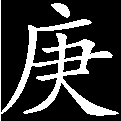
\includegraphics[width=3mm]{../Images/00004}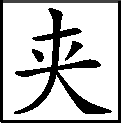
\includegraphics[width=3mm]{../Images/00012}\footnotesize \kaishu 可知放账乃发,所谓此家儿知耻恶之事也。}\href{../Text/part0076_split_000.html\#lnkback_3_a}{\textsuperscript{③}}既这样,我就收了回来。我比谁不会花钱,咱们以后就坐着花,到多早晚是多早晚。这不是样儿:前儿老太太生日,太太急了两个月,想不出法儿来,还是我提了一句,后楼上现有些没要紧的大铜锡家伙四五箱子,拿去弄了三百银子,才把太太遮羞礼儿搪过去了。我是你们知道的,那一个金自鸣钟卖了五百六十两银子。没有半个月,大事小事倒有十来件,白填在里头。今儿外头也短住了,不知是谁的主意,搜寻上老太太了。明儿再过一年,各人搜寻到头面衣服,可就好了!''旺儿媳妇笑道:``那一位太太奶奶的头面衣服折变了不够过一辈子的,只是不肯罢了。''{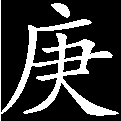
\includegraphics[width=3mm]{../Images/00004}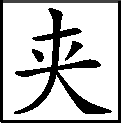
\includegraphics[width=3mm]{../Images/00012}\footnotesize \kaishu 闲语,补出近日诸事。}凤姐道:``不是我说没了能耐的话,要像这样,我竟不能了。昨晚上忽然作了一个梦,说来也可笑,{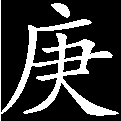
\includegraphics[width=3mm]{../Images/00004}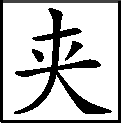
\includegraphics[width=3mm]{../Images/00012}\footnotesize \kaishu 反说``可笑'',妙甚!若必以此梦为凶兆,则思反落套,非红楼之梦矣。}梦见一个人,虽然面善,却又不知名姓,{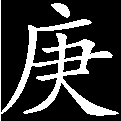
\includegraphics[width=3mm]{../Images/00004}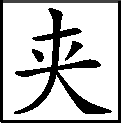
\includegraphics[width=3mm]{../Images/00012}\footnotesize \kaishu 是以前授方相之旧,数十年后矣。}找我。问他作什么,他说娘娘打发他来要一百匹锦。我问他是那一位娘娘,他说的又不是咱们家的娘娘。我就不肯给他,他就上来夺。正夺着,就醒了。''{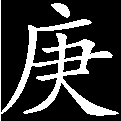
\includegraphics[width=3mm]{../Images/00004}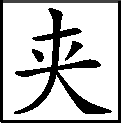
\includegraphics[width=3mm]{../Images/00012}\footnotesize \kaishu 妙!实家常触景闲梦,必有之理,却是江淹才尽之兆也,可伤。}旺儿家的笑道:``这是奶奶的日间操心,常应候宫里的事。''{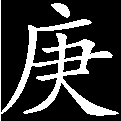
\includegraphics[width=3mm]{../Images/00004}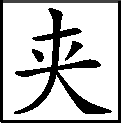
\includegraphics[width=3mm]{../Images/00012}\footnotesize \kaishu 淡淡抹去,妙!}

一语未了,人回:``夏太府打发了一个小内监来说话。''贾琏听了,忙皱眉道:``又是什么话,一年他们也搬够了。''凤姐道:``你藏起来,等我见他,若是小事罢了,若是大事,我自有话回他。''贾琏便躲入内套间去。这里凤姐命人带进小太监来,让他椅子上坐了吃茶,因问何事。那小太监便说:``夏爷爷因今儿偶见一所房子,如今竟短二百两银子,打发我来问舅奶奶家里,有现成的银子暂借一二百,过一两日就送过来。''{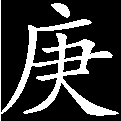
\includegraphics[width=3mm]{../Images/00004}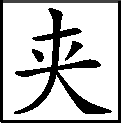
\includegraphics[width=3mm]{../Images/00012}\footnotesize \kaishu 可谓``密处不容针''。}凤姐儿听了,笑道:``什么是送过来,有的是银子,只管先兑了去。改日等我们短了,再借去也是一样。''小太监道:``夏爷爷还说了,上两回还有一千二百两银子没送来,等今年年底下,自然一齐都送过来。''凤姐笑道:``你夏爷爷好小气,这也值得提在心上。我说一句话,不怕他多心,若都这样记清了还我们,不知还了多少了。只怕没有,若有,只管拿去。''因叫旺儿媳妇来,``出去不管那里先支二百两来。''旺儿媳妇会意,因笑道:``我才因别处支不动,才来和奶奶支的。''凤姐道:``你们只会里头来要钱,叫你们外头算去就不能了。''说着叫平儿,``把我那两个金项圈拿出去,暂且押四百两银子。''平儿答应了,去半日,果然拿了一个锦盒子来,里面两个锦袱包着。打开时,一个金累丝攒珠的,那珍珠都有莲子大小,一个点翠嵌宝石的。两个都与宫中之物不离上下。{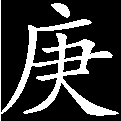
\includegraphics[width=3mm]{../Images/00004}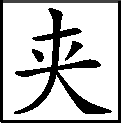
\includegraphics[width=3mm]{../Images/00012}\footnotesize \kaishu 是太监眼中看、心中评。}一时拿去,果然拿了四百两银子来。凤姐命与小太监打叠起一半,那一半命人与了旺儿媳妇,命他拿去办八月中秋的节。{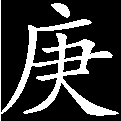
\includegraphics[width=3mm]{../Images/00004}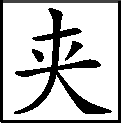
\includegraphics[width=3mm]{../Images/00012}\footnotesize \kaishu 过下伏脉。}那小太监便告辞了,凤姐命人替他拿着银子,送出大门去了。这里贾琏出来笑道:``这一起外祟何日是了!''凤姐笑道:``刚说着,就来了一股子。''贾琏道:``\elegantpar{昨儿周太监来,张口一千两。我略应慢了些,他就不自在。将来得罪人之处不少。这会子再发个三二百万的财就好了。}{盘根错节}''一面说,一面平儿伏侍凤姐另洗了面、更衣,往贾母处去伺候晚饭。

这里贾琏出来,刚至外书房,忽见林之孝走来。贾琏因问何事。林之孝说道:``方才听得雨村降了,却不知因何事,只怕未必真。''贾琏道:``真不真,他那官儿也未必保得长。将来有事,\href{../Text/part0076_split_000.html\#lnkback_4_a}{\textsuperscript{④}}怕咱们宁可疏远着他好。''林之孝道:``何尝不是,只是一时难以疏远。如今东府大爷和他更好,老爷又喜欢他,时常来往,那个不知。''贾琏道:``横竖不和他谋事,也不相干。你去再打听真了,是为什么。''林之孝答应了,却不动身,坐在下面椅子上,且说些闲话。因又说起家道艰难,便趁势又说:``人口太重了。不如拣个空日回明老太太老爷,把这些出过力的老家人用不着的,开恩放几家出去。一则他们各有营运,二则家里一年也省些口粮月钱。再者里头的姑娘也太多。俗语说:`一时比不得一时。'如今说不得先时的例了,少不得大家委屈些,该使八个的使六个,该使四个的便使两个。若各房算起来,一年也可以省得许多月米月钱。况且里头的女孩子们一半都太大了,也该配人的。\elegantpar{配人成了房,岂不又孳生出人来。}{他是觉得配人好,还是不配好?}''贾琏道:``我也这样想着,只是老爷才回家来,多少大事未回,那里议到这个上头。前儿官媒拿了个庚帖来求亲,太太还说老爷才来家,每日欢天喜地的说骨肉完聚,忽然就提起这事,恐老爷又伤心,所以且不叫提这事。''林之孝道:``这也是正理,太太想的周到。''

贾琏道:``正是,提起这话我想起了一件事来。我们旺儿的小子要说太太房里的彩霞。他昨儿求我,我想什么大事,不管谁去说一声去。这会子有谁闲着,你打发个人去说一声,就说我的话。''\href{../Text/part0076_split_000.html\#lnkback_5_a}{\textsuperscript{⑤}}林之孝听了,只得应着,半晌笑道:``依我说,二爷竟别管这件事。旺儿的那小儿子虽然年轻,在外头吃酒赌钱,无所不至。虽说都是奴才们,到底是一辈子的事。彩霞那孩子这几年我虽没见,听得越发出挑的好了,何苦来白糟踏一个人。''贾琏道:``他小儿子原会吃酒,不成人?''林之孝冷笑道:``岂只吃酒赌钱,在外头无所不为。我们看他是奶奶的人,也只见一半不见一半罢了。''贾琏道:``我竟不知道这些事。既这样,那里还给他老婆,且给他一顿棍,锁起来,再问他老子娘。''林之孝笑道:``何必在这一时。那是错也等他再生事,我们自然回爷处治。如今且恕他。''贾琏不语,一时林之孝出去。

晚间,凤姐已命人唤了彩霞之母来说媒。那彩霞之母满心纵不愿意,见凤姐亲自和他说,何等体面,{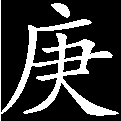
\includegraphics[width=3mm]{../Images/00004}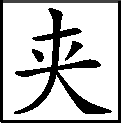
\includegraphics[width=3mm]{../Images/00012}\footnotesize \kaishu 今时人因图此现在体面,误了多少女儿,此正是为今时女儿一{(笑)}{[}哭{]}。}便心不由意的满口应了出去。今凤姐问贾琏可说了没有,贾琏因说:``我原要说的,打听得他小儿子大不成人,故还不曾说。若果然不成人,且管教他两日,再给他老婆不迟。''凤姐听说,便说:``你听见谁说他不成人?''贾琏道:``不过是家里的人,还有谁。''凤姐笑道:``我们王家的人,连我还不中你们的意,何况奴才呢。我才已竟和他母亲说了,他娘已经欢天喜地应了,难道又叫进他来不要了不成?''贾琏道:``既你说了,又何必退,明儿说给他老子好生管他就是了。''这里说话不提。

且说彩霞因前日出去,等父母择人,心中虽是与贾环有旧,尚未作准。今日又见旺儿每每来求亲,早闻得旺儿之子酗酒赌博,而且容颜丑陋,一技不知,自此心中越发懊恼。生恐旺儿仗凤姐之势,一时作成,终身为患,不免心中急躁。遂至晚间悄命他妹子小霞{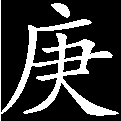
\includegraphics[width=3mm]{../Images/00004}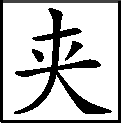
\includegraphics[width=3mm]{../Images/00012}\footnotesize \kaishu 霞大小,奇奇怪怪之文,更觉有趣。}进二门来找赵姨娘,问了端的。

赵姨娘素日深与彩霞契合,巴不得与了贾环,方有个膀臂,不承望王夫人又放了出去。每唆贾环去讨,一则贾环羞口难开,二则贾环也不大甚在意,不过是个丫头,他去了,将来自然还有,{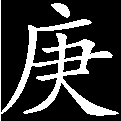
\includegraphics[width=3mm]{../Images/00004}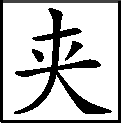
\includegraphics[width=3mm]{../Images/00012}\footnotesize \kaishu 这是世人之情,亦是丈夫之情。}遂迁延住不说,意思便丢开。无奈赵姨娘又不舍,又见他妹子来问,是晚得空,便先求了贾政。{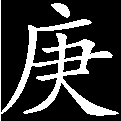
\includegraphics[width=3mm]{../Images/00004}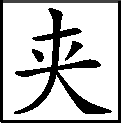
\includegraphics[width=3mm]{../Images/00012}\footnotesize \kaishu 这是使人想不到之文,却是大家必有之事。}贾政因说道:``且忙什么,等他们再念一二年书再放人不迟。我已经看中了两个丫头,一个与宝玉,一个给环儿。只是年纪还小,又怕他们误了书,所以再等一二年。''{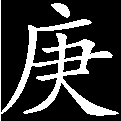
\includegraphics[width=3mm]{../Images/00004}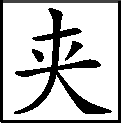
\includegraphics[width=3mm]{../Images/00012}\footnotesize \kaishu 妙文。又写出贾老儿女之情。细思一部书总不写贾老,则不成文,若不如此写,则又非贾老。}赵姨娘道:``宝玉已有了二年了,老爷还不知道?''贾政听了忙问道:``谁给的?''赵姨娘方欲说话,只听外面一声响,不知何物,大家吃了一惊不小。要知端的,且听下回分解。

{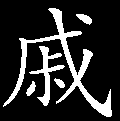
\includegraphics[width=3mm]{../Images/00005}\kaishu 总评:夏雨冬风,常不解其何自来、何自去?鸳鸯与司棋相哭发誓,事已瓦释冰消,及平地风波一起,措手不及,亦不解何自来、何自去。}

%{  \href{../Text/part0076_split_000.html\#navto_1_a}{①}``家亲'',原指已故的亲人,义同``家神''。《地藏菩萨本愿经·如来赞叹品第六》:``或夜梦恶鬼,乃及家亲。''这里借喻``内鬼''。俗语有``家(内)神通外鬼''之语,意即内外勾结。}
%
%{  \href{../Text/part0076_split_000.html\#navto_2_a}{②}``也要'',蒙、戚本作``不要'',意思相反。究竟该``要''还是``不要'',原因在于对俗语``前人撒土迷了后人的眼''的理解分歧。按《金瓶梅词话》第八十回:(应伯爵道:)``今日他(西门庆)没了,莫非推不知道?洒土也眯了后人眼睛儿也。''又,清李光庭《乡言解颐》卷一:``前人撒土眯后人眼,谓含糊了事也。''由此可见,``前人撒土迷了后人的眼''是个歇后语,``前人撒土''是引子,``迷了后人的眼''才是本意:遮掩后人的眼睛,做做样子给人看。因此此处应以``也要''为是。从书中前后叙述和凤姐话意,都看不出有``隆重''去给尤二姐上坟的意思。}
%
%{\href{../Text/part0076_split_000.html\#navto_3_a}{③}``可知放账乃发,所谓此家儿知耻恶之事也。''此语读来不很通畅,意思还大体明白:虽然放高利贷可以发财,但这是连家下童仆都知道羞耻的事情。``此家儿知耻恶''前加``所谓''二字,则此语似为引用,或另有出处。有研究者以形讹校改``乃''、``儿''二字,成为``可知放账事发,所谓此家鬼知耻恶之事也。''意思全变,而文句并不变得更通畅。因``放账事发''涉及佚稿问题,不可证伪。兹不采纳。}

% {\href{../Text/part0076_split_000.html\#navto_4_a}{④}此处从底本原文。``将来有事'',联系上下文,当理解为``我们家将来有事'',诸本均作``雨村将来要出事''解,因而各补充若干字以足文义,非是。}

% {\href{../Text/part0076_split_000.html\#navto_5_a}{⑤}原作``这会子有谁闲着,我打发个人去说一声,就说我的话'',诸本(除蒙本外)均同。蒙本作``这会子谁去呢?你闲着,就打发个人去说一声'',语虽不佳,``打发个人去''的是``你''不是``我'',是对的。按贾琏既认为这是小事,自不必亲自派人,让林之孝随便打发个闲着的人去说,``就说我的话''就足够了。下文``林之孝听了,只得应着''可证。现酌参蒙本改``我''为``你''字。}
